\documentclass[a4paper,10pt]{article}

\addtolength{\hoffset}{-2.5cm}
\addtolength{\textwidth}{5cm}
\setlength{\headheight}{13pt}
\addtolength{\voffset}{-1.5cm}
\addtolength{\textheight}{3.5cm}

\usepackage{hyperref}
\usepackage{tikz}

\usetikzlibrary{er}

\hypersetup{pdftitle=ER-Diagramm - Android-App}
\author{Oliver Braunsdorf \and Vanessa Gries \and Chris Köcher}
\title{ER-Diagramm - Android-App}
\date{\today}


\begin{document}
\begin{center}
 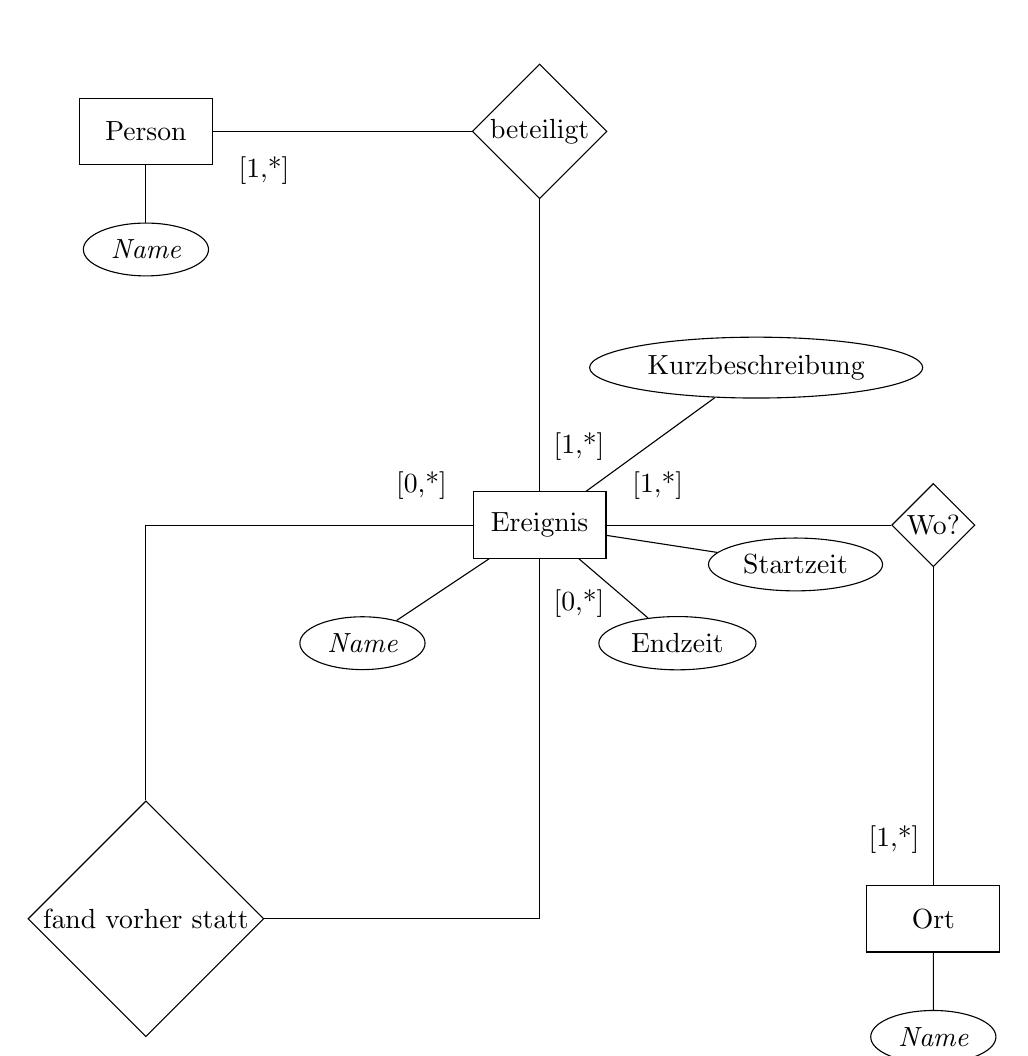
\begin{tikzpicture}
  \node[entity] (event) at (5,5) {Ereignis}
       child {node[key attribute] at (0,0) {Name}}
       child {node[attribute] at (4,1) {Startzeit}}
       child {node[attribute] at (1,0) {Endzeit}}
       child {node[attribute] at (0.5,3.5) {Kurzbeschreibung}}
       edge (0,5)
       edge (5,0);
  \node[entity] (ort) at (10,0) {Ort}
       child {node[key attribute] at (0,0) {Name}};
  \node[entity] (person) at (0,10) {Person}
       child {node[key attribute] at (0,0) {Name}};
  \node[relationship] (bet) at (5,10) {beteiligt}
       edge (event)
       edge (person);
  \node[relationship] (wo) at (10,5) {Wo?}
       edge (event)
       edge (ort);
  \node[relationship] (vorg) at (0,0) {fand vorher statt}
       edge (0,5)
       edge (5,0);
  \node at (5.5,4) {[0,*]};
  \node at (3.5,5.5) {[0,*]};
  \node at (6.5,5.5) {[1,*]};
  \node at (9.5,1) {[1,*]};
  \node at (5.5,6) {[1,*]};
  \node at (1.5,9.5) {[1,*]};
 \end{tikzpicture}
\end{center}
\end{document}